\chapter{\textit{Grasp}について}
\label{graspについて}

第\ref{related_works}章では、「身体化」に関する先行研究について、それぞれの分野でどのように展開しているのかについてを概観し、その中での本研究の位置付けと貢献を示した。

本章では、本研究における「人馬一体」といった関係性についてより詳細に捉えるため、Sydney Felsによるembodimentの分類を導入する。
そして、身体化過程における意識的な試行期間を捉える新たな概念として\textit{grasp}を提示する。その上で、Felsの分類との関係性と、この概念を用いることから修士作品の体験についてのねらいを説明する。また、この概念に至るまでのプロトタイピングの過程を示すことで、この概念を主張する根拠とする。

\section{Felsのembodiment}
コンピューター工学の研究者であるSydney Felsは2000年、「Intimacy and Embodiment: Implications for Art and Technology」\cite{Fels}において、人間と対象との関係性を「embodiment」の観点から4つのカテゴリに分類した。
それぞれの説明は以下の通りである(括弧内は筆者訳)。

\textbf{Response(応答):}\\
対象に対する働きかけの結果から、感情的な反応や理解を得る状態を指す。Felsはこの関係性の例として「コンピュータとそれに初めて触れた人」を挙げ、「なんらかの操作を通して得られた、便利な機能に喜んでいる状態、また逆に「有用な結果を得られず落胆する状態」と説明する。

\textbf{Control(制御):}\\
人が対象を自分自身の延長として使用し、その操作によって感情的な満足や美的体験を得る状態を指す。例えばピアノの演奏において、「音が出ている」ということだけでなく、自分自身の表現したいことが、不自由なくピアノを通して体現されていると感じるときの、一体感によってもたらされる心地よさがこれに該当する\footnote{「Control」においてFelsは、「自分自身の延長」として経験される感覚であり、またそれが追従性の高いグラフィックによってもたらされると説明する。これは、渡邊がマウスカーソルやスマートフォンに対して用いた「操作時の指とグラフィックの追従性が高い」インターフェースという説明と同等のものであると考えられる。このことからFelsの分類におけるControlは、渡邊の「自己帰属感」と重なる。}。

\textbf{Contemplation(鑑賞):}\\
人が対象に対して働きかけることはないが、人がその対象からの信号やメッセージを内省や反映を通じて、感情的になったり美的体験を得る状態を指す。Felsはその具体例として、絵画の鑑賞体験を挙げる。

\textbf{Belonging(帰属):}\\
対象によって人が動かされているような経験を指す。人はその対象によって提供される体験を通じて感情的な反応を得る。ここでは、対象が人の体験や感情を形作る役割を果たす。たとえばバイクの運転において、「バイクに合わせた走り方をする」といったように、単にその対象を通して使い手の意図がそのまま体現されるのではなく、その対象に合わせた振る舞いがそこで形作られることに喜びを見出すような状態である。

\begin{figure}[H]
  \centering
  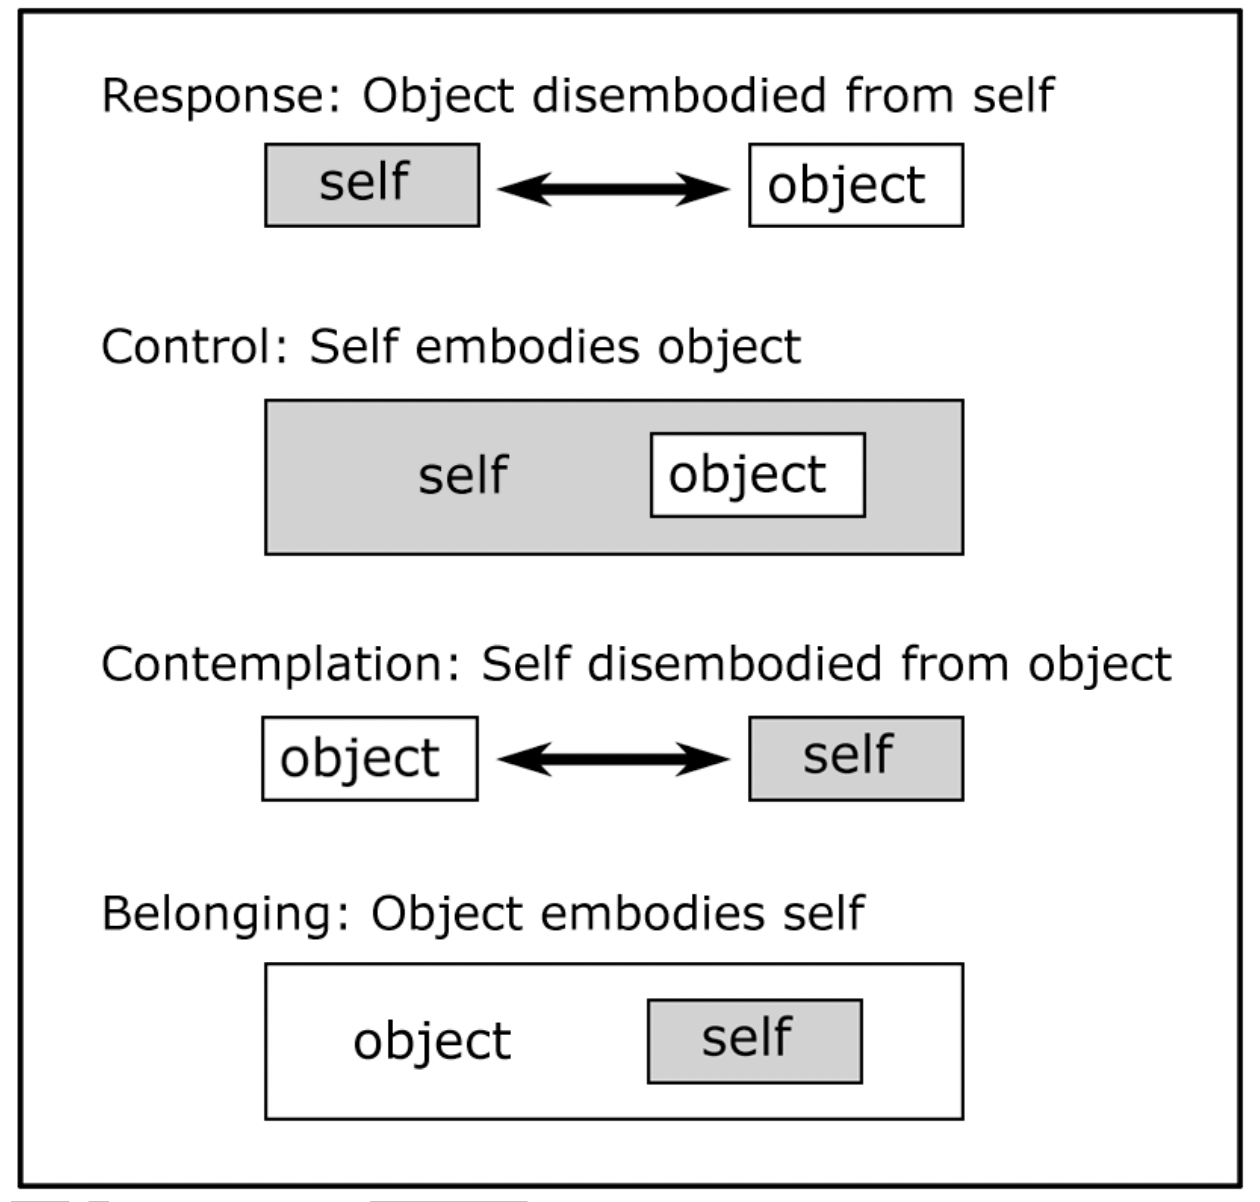
\includegraphics[width=8cm]{img/fels_diagram.png}
  \caption{Felsによるembodiment(仮置き)}
  \label{fig:fels_embodiment}
\end{figure}

% さて、Felsは特に、上記「制御 Control」においては「自分自身の延長」として経験される感覚について言及しており、またそれが追従性の高いグラフィックによってもたらされるという記述は、渡邊がマウスカーソルやスマートフォンに対して用いた「操作時の指とグラフィックの追従性が高い」インターフェースという説明と同等のものである。このことからFelsのいうControlとは、Gallagherの「sense of ownership」と同じものを指していると考えられる。その上で、embodimentの状態をControlのみならずBelongingから捉えていること、そしてembodimentが生じていない状態についても言及していることなど、現在HCIの分野で一般に用いられる意味でのembodimentよりも広く、人と対象を捉えるモデルとなっていることが確認できる。

% さらにFelsは、対象と人とのあいだにある「深い関係」を指して、「Intimacy」という尺度で説明する。例えば楽器と人の関係性ように、Intimacyのある関係性のもとでは、「あたかもその装置が身体の延長であるかのように、考えや感情を効果的に表現できる」という。上記の、Felsによるembodimentの分類においては、ResponseがIntimacyの低い状態、ControlがIntimacyの高い状態として説明される。

他者性と向き合う中で、自分なりの扱い方を見出すことは、Felsの分類における「Belonging」であると言える。しかしこの状態であっても、「Control」も同時に行われている。またFelsは、自分の意志と対象の制約や他者性とのあいだで折り合いをつけることで得られる「親密な関係」を、「Intimacy」という言葉で説明した\footnote{"\textit{Intimacy deals with the subjective match between the behaviour of a device and the operation of that device.}"Fels(2000)\cite{Fels}より}。

このことから、本研究が目指す「人馬一体」という言葉をFelsの用語を用いると、
\begin{quote}
  「Control」と「Belonging」が両方生起することで生じる「Intimacy」  
\end{quote}
と説明できる。しかし、Felsはこうした分類を行ったが、それらがどのようにして生起するかについては述べていない。そこで、本研究では次節に定義する\textit{grasp}こそが、その生起に重要な役割を果たしているのではないかという仮説を立てた。


\section{\textit{grasp}の定義}
\label{grasp_difinition}
\textit{grasp}について、本研究では次のように定義する。

\begin{quote}
  \textbf{人と対象との関係の中で、人が対象の中に注意や目的意識を抱きながら、意識的に試行する期間}
\end{quote}

graspは「把握」を意味する動詞でもあるが、ここで「動作」ではなく「期間」とした。その理由は、「意識的に試行する」とき、同時にその結果を受けて気づきを得たり、その気づきをもとに新たな関心を抱くといった、単に自分が行為しているだけではなく、対象から影響を受けながら次の行為が決まってくるようなフィードバックループの構造があると考えるためである。「grasp=把握」という言葉についても、単に「ものを掴む」という意味だけでなく、「理解」の意味があることは、対象について一方向に働きかけているのではない様子が現れているのではないだろうか。

\textit{grasp}とは例えば、ギターの習得過程において、弾きこなしたいフレーズを定め、それを達成するまでに試行錯誤をし、達成できるようになるまでの期間である。熟達した状態では、熟達する前とは違う視座でものごとを捉えられるようになり、また違う対象に注意が向くようになると、ギターと人との間に別の\textit{grasp}が芽生える。
またあるいは、\textit{grasp}の過程で、対象と向き合い続ける過程の中でその解像度が高まり、当初目指していたこととは違うことに興味を抱く(セレンディピティ)ことでも、別の\textit{grasp}が芽生える。

ここまで具体例を通してみてきたように、\textit{grasp}は、ギターと人との関係において一度だけ生じるのではなく、注目する対象が定まれば何度でも生じる。
% ここで、\textit{grasp}は人と対象の関係の中で、人が注意を向ける「対象」ごとに別の\textit{grasp}があると言えそうだが、注意を向けている「対象」がなんであるか、断言できなかったり、本人も判然としないこともある。そのため、


\section{Felsの議論との関係性}
ここでは\textit{grasp}が、FelsのEmbodimentとどう関係するのかについて説明する。
先の節\ref{grasp_difinition}に挙げたように、人は\textit{grasp}を通して、あるいはその過程で、対象から影響を受けながら次の試行が形作られていく。この時の「試行」には、挙動を確かめるような動作、すなわちFelsの「Response」もあれば、試行を通して得られた結果をもとに、何かに考えを巡らす「Contemplation」も含まれる。こうした試行の積み重なりから、人と対象のあいだに「Control」や「Belonging」の関係、すなわちFelsの意味でのEmbodimentが生じるのではないか。

つまりこの概念は、折り合いをつけていくまでの「間」に行われていることについて語ることを可能にするものである。\textit{grasp}の様相を捉えることで、現状からEmbodimentが達成されるまでのあいだに欠けているものが何であるかを語る術を得られるのではないか、と考える。

\section{\textit{grasp}を踏まえたIntimacyが起こるまでの過程についての仮説}
\textit{grasp}が、本研究の関心である「対象からの影響も受けつつ(Belonging)、相互の折り合いをつけながら生まれる一体感(Intimacy)が起こる」までの過程に必要ではないか、と考える。

そしてそのためには、注意を向ける対象や目的意識を抱く対象が変わりながらも\textit{grasp}が継続していく体験が良いのか、それとも注意を向ける対象は変わらず、1つのものに対する目的意識が長く継続し、\textit{grasp}も長い体験が良いのか。このいずれであるかが判別することができれば、より詳細にこの体験を説明することができると考えた。

\section{プロトタイピング}
本研究では、手指の変換表現を通して\textit{grasp}が生じる表現や構成を探索した。
最終的な作品形態に至るまでに、総計60パターンのプロトタイプ制作を行なった。プロトタイピングにおける目的を時系列で3段階に大別すると、「テーマの着想」、「変換表現についての探索」、そして「表現の収束」である。「テーマの着想」に至るまでのプロトタイピングについては、\ref{prototyping_concept_making}節にて説明した。ここでは、後の2つについて説明する。

手指の変換表現の中でも、単に形を考えるだけでなく、どの動きをその形に当てはめるか、そしてどの時間の動きを用いるか等、さまざまな変換方法が考えられる。この段階では先入観によって絞り込むことがないよう、このような探索空間の中で思いつく限り実装し、実際に体験することを通して判断するという姿勢でプロトタイピングをおこなった。以下では、行ったプロトタイピングについて、「形状」、「構造」、「時間操作」の観点から分類する。その上で、これらのプロトタイピングを通してどのような知見を得て、次の探索へつながったのかについての説明を「振り返り」としてこの節の最後に述べる。

\subsection{形状}
形状については、指を動きの最小単位として、指ごとに独立したバリエーション、指同士を直列に繋ぎ合わせたバージョン、円形に繋ぎ合わせたバージョンなどを作成した。また、単位である指をどのように表現するかについては、「円形」、「くの字」、「ひょうたん型」などのバリエーションで表現を試みた。
\begin{figure}[H]
  \centering
  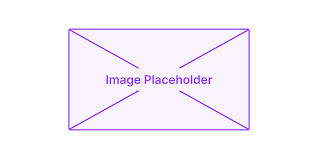
\includegraphics[width=15cm]{img/placeholder.png}
  \caption{ユニットのバリエーション}
  \label{fig:unit_valiation}
\end{figure}
\subsection{マッピングの方法}
マッピングについては、1つの動きを複製して、1つの動きを複数のパーツの動きへと波及させるバリエーションなどを作成した。図\ref{fig:networked_finger}に示すプロトタイプ\footnote{\url{https://eee-handpose-playground.vercel.app/work/createNetworkedFingers}}では、指先をクリックすると5本ある指のうちのいずれかの動きを追従する指が、指先に追加されるものである。どの指が付け加わるかはランダムで、指が新しく追加されるたびに、それがどの指の運動であるかを同定するには、一本一本指を動かして、どこがその指に対応しているのかについて同定する必要がある。

またそのほかに、図\ref{fig:fractal_finger}に示すプロトタイプ\footnote{\url{https://eee-handpose-playground.vercel.app/work/fractalFingers}}では、親指の先に人差し指の動きが複数分岐し、さらに人差し指の先から中指の動きが複数分岐して配置される、といったフラクタル構造で指の動きを配置したパターンを制作した。このように、配置を変えるだけでなく1つの指の動きに対して対応して動く部分を多数にするなどのバリエーションを検討した。

\begin{figure}[htbp]
  \begin{minipage}[b]{0.5\linewidth}
    \centering
    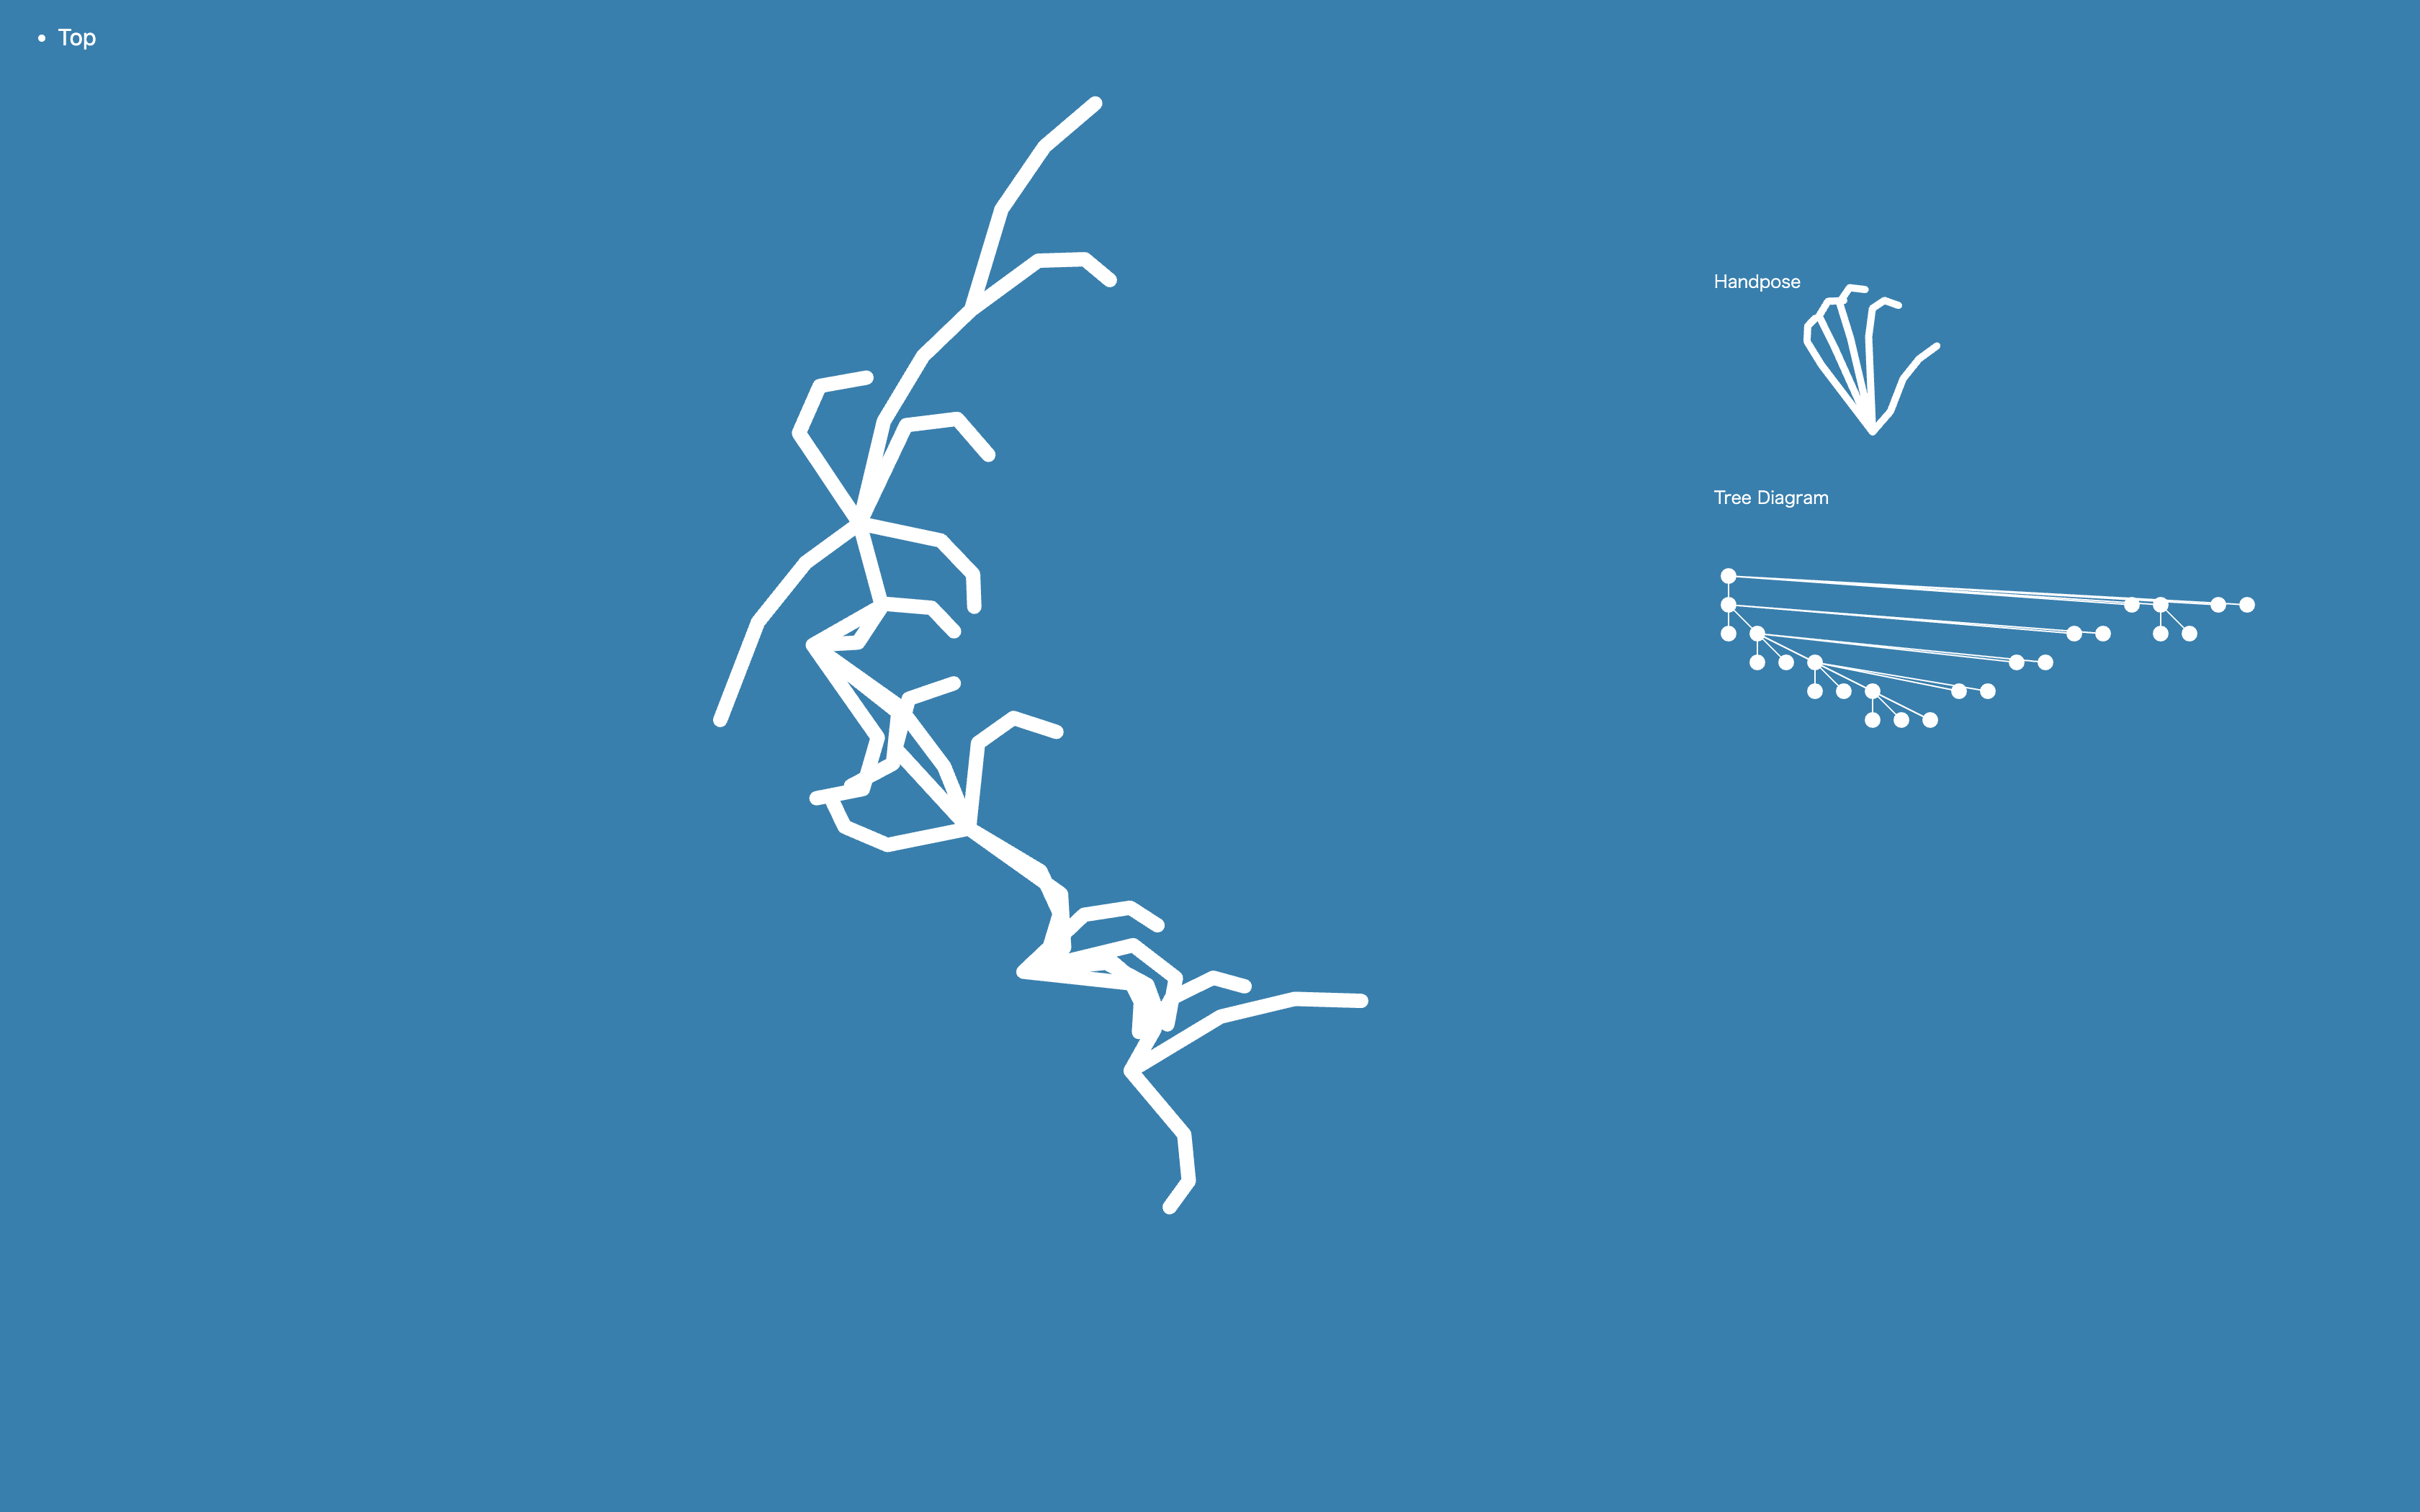
\includegraphics[keepaspectratio, width=7cm]{img/networked_finger.png}
    \caption{Networked Finger}
    \label{fig:networked_finger}
  \end{minipage}
  \begin{minipage}[b]{0.5\linewidth}
    \centering
    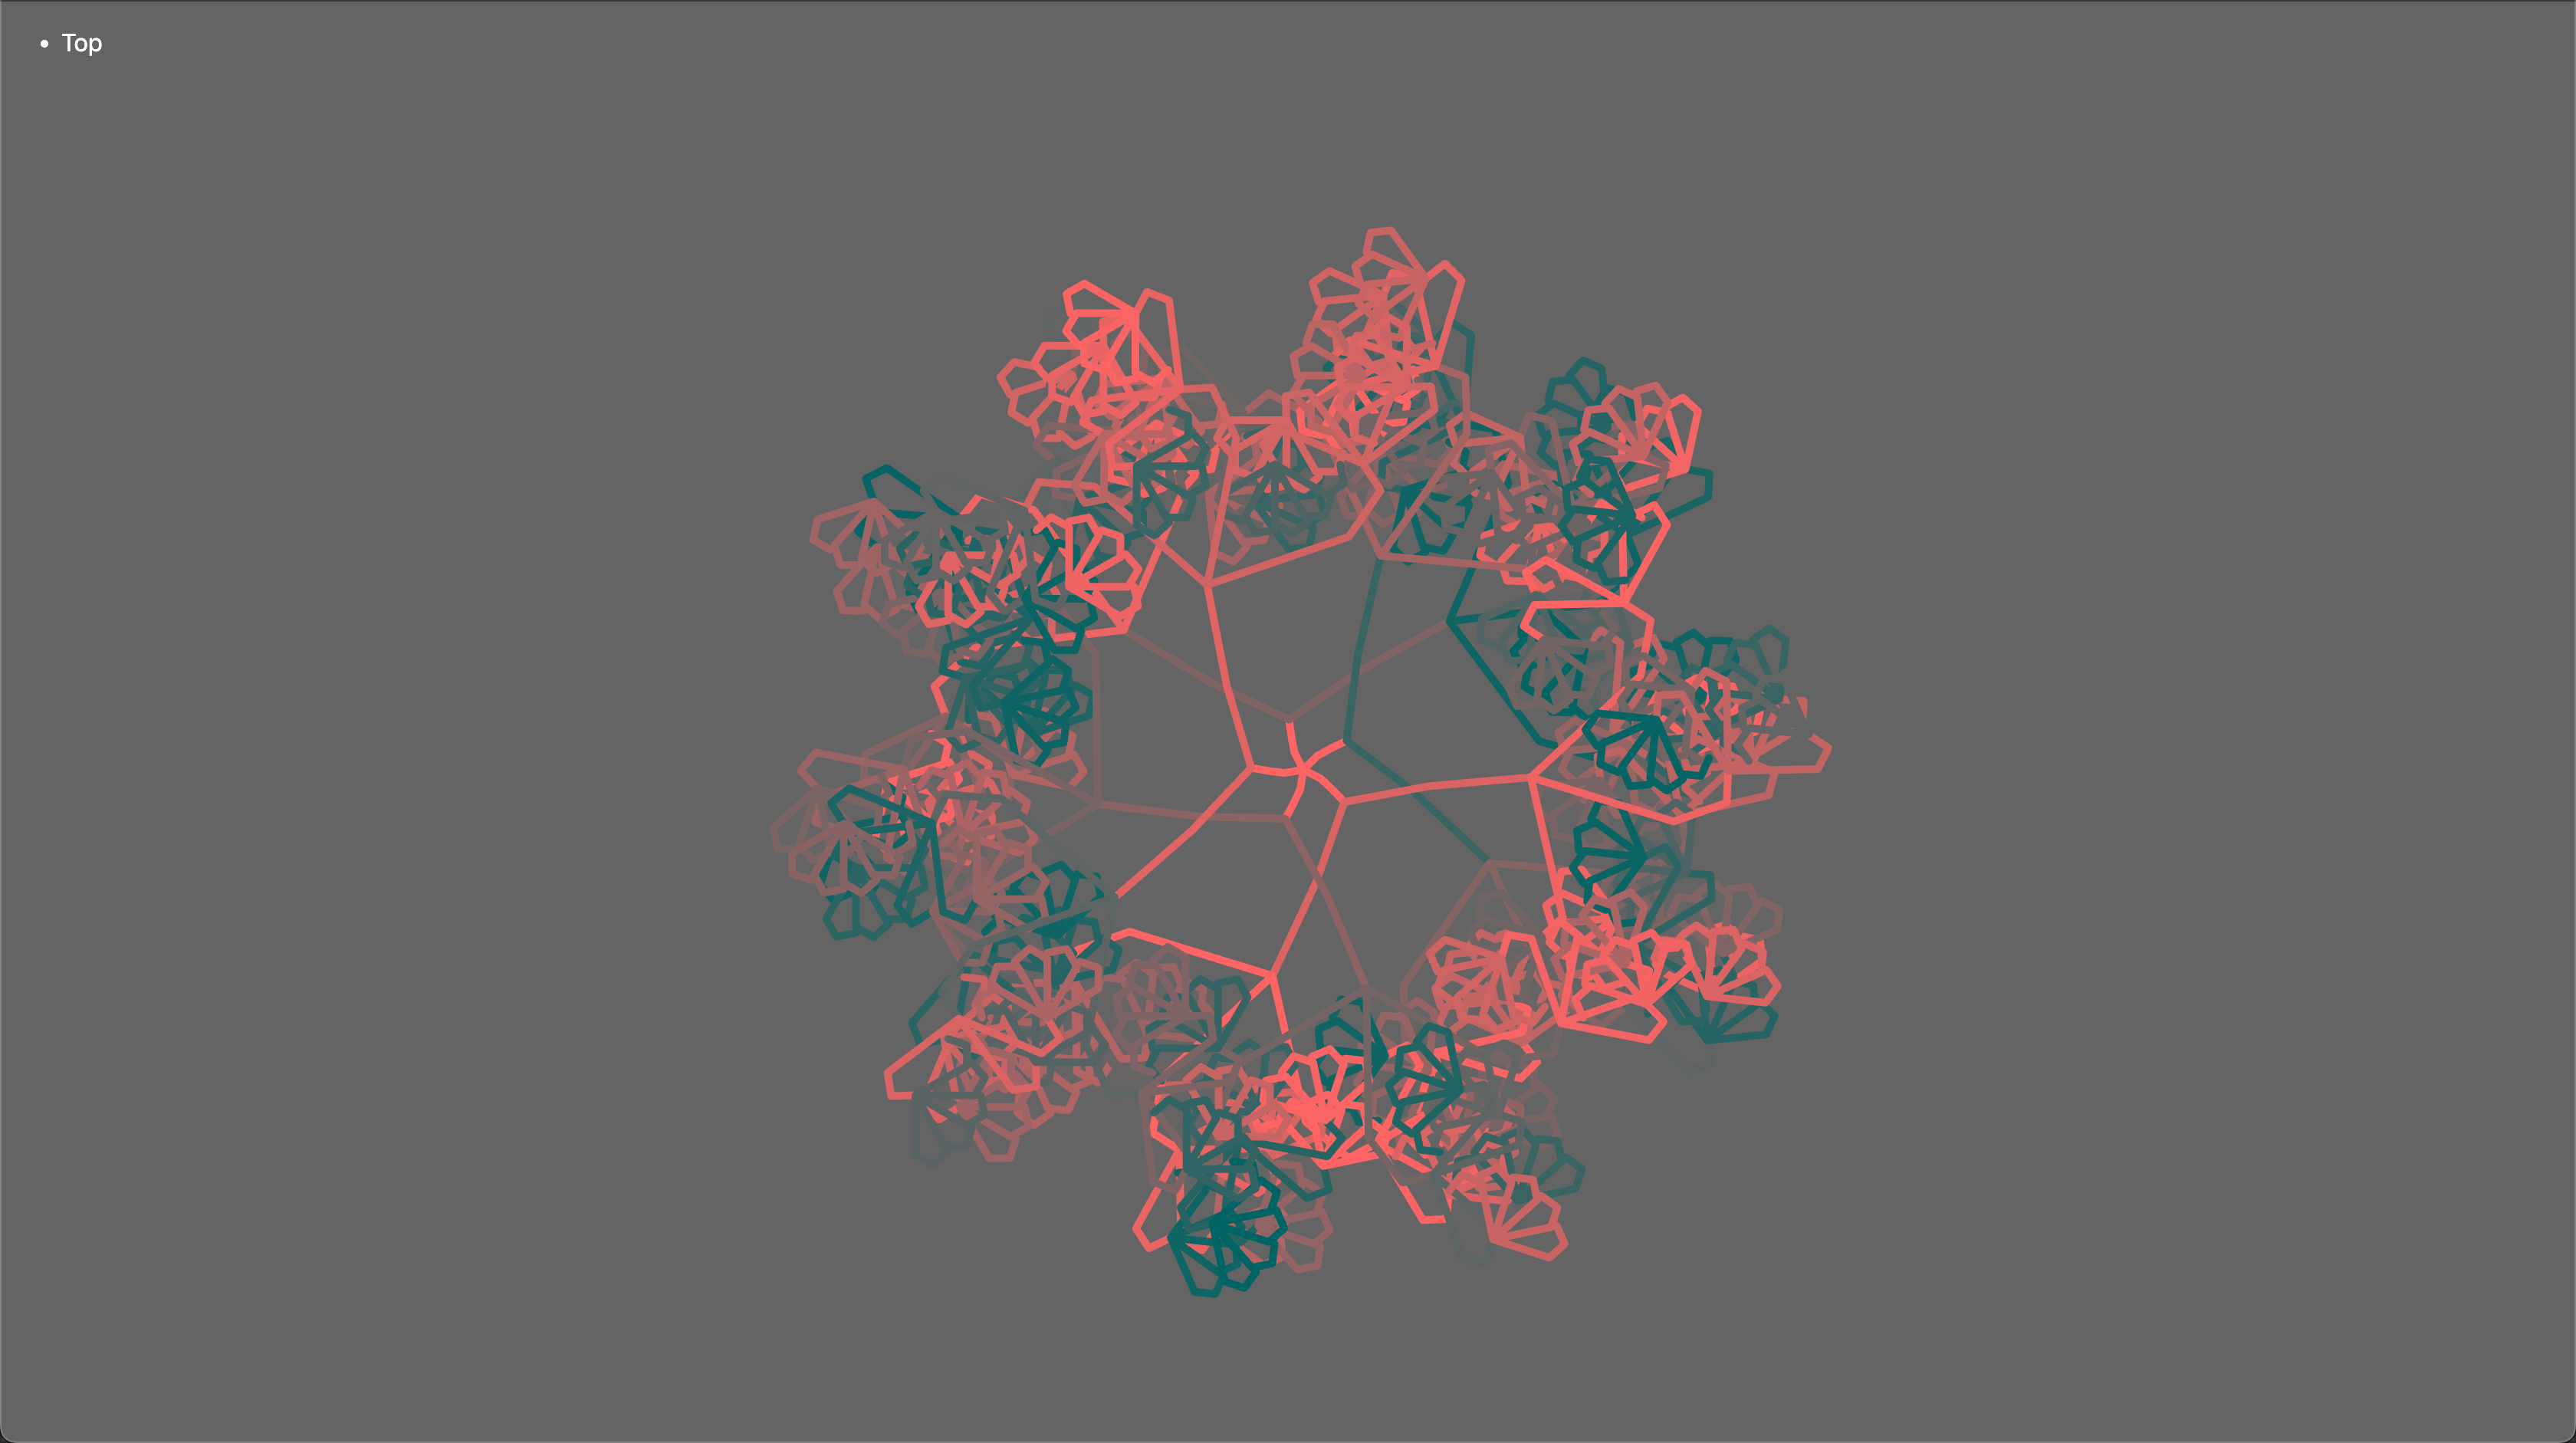
\includegraphics[keepaspectratio, width=7cm]{img/fractel_finger.png}
    \caption{Fractal Finger}
    \label{fig:fractal_finger}
  \end{minipage}
\end{figure}
\subsection{時間操作}
最新の自分の動きだけを表示するのではなく、過去の動きも表示するプロトタイプにも取り組んだ。図\ref{fig:prototype_delay}に示すプロトタイプでは、5本の指の動きが等間隔に並べられているが、それぞれの指は、鉛直上向きの角度に現在の指の動き、そこから時計回りに、順次過去の指の動きが並べられている\footnote{\url{https://interaction005-moe5dbh11-k1105.vercel.app/}}。

\begin{figure}[H]
  \centering
  
\includegraphics[width=15cm]{img/past_time.png}
  \caption{過去の動きを用いた例}
  \label{fig:prototype_delay}
\end{figure}

このプロトタイプでは、指先を小さく動かすと、その動きが時計回りに伝播していくようすが見て取れる。これは例えばゼリー状の物体を触れた時のような、衝撃が物体全体へと伝播していくようすに見立てられるため、柔らかいオブジェクトに触れているときのような身体感覚を錯覚することがある。

\subsection{ボール操作(執筆中)}
単に変換するだけでなく、ボール操作のような

\subsection{振り返り(執筆中)}
形状については、円形、くの字、ひょうたん型などの変換を試みたが、動きに対して注意が向けられたのは「くの字」の形状であると感じられた。この理由について、身体動作である指の折り曲げとの対応から考察する。身体動作として指の折り曲げが画面の中で、円の半径へと対応している場合とくの字のような折り曲げ動作に反応している場合とを比べたとき、後者は実際には指先と指の付け根の距離しか評価していないにも関わらず、制御点が3つあるように感じられる。そう捉えると、円の半径が変化していくことよりも対応関係が厳密であり、それを動かすことによって得られる心地よさは、Felsの「Control」による心地よさであると捉えられる。その一方で、円の半径に関節の動きをマッピングさせるような表現については、縮んだり、膨らんだりする動きには共感しづらい。微細な運動が増幅される「気持ちよさ」があるが、この気持ちよさは身体動作との連動によってもたらされる気持ちよさではなく、動作に対するフィードバックに対する快、すなわちFelsのいう「Response」による快が強い。

また、マッピング方法に関しては、1つの指の動きがフラクタル的に配置する場合について、動きの複雑度が上がっているにも関わらず、感覚としてはより単純な動きであると感じられた。これについては、グラフィックデザイナーの女性が体験した際「構造としては緻密であるのに、動きは単純であるように感じる」と意見した。その理由として彼女は、「対称性が前面に出ているため、シンボルとしての印象を強く感じてしまう」「意識していないところも同時に動いている感覚があるため、自分の動きだと思えない」からではないかと推測した。このことから、手指の複数ある制御点の数よりも、多すぎる表現も、少なすぎる表現も、運動に対する共感性は下がり、「Control」の感覚よりも「Response」の感覚のほうが強くなるのではないかと考察する。

時間操作については、やわらかい


\section{選定と作品構成}
ここまで説明したプロトタイピングと振り返りを踏まえて、最終的な作品構成へ繋がる評価軸や、採用された構成について説明する。
\subsection{動かしている感覚が強い表現}
1つ目の観点として、手指の微細かつ複雑な動きをもって、緻密な制御をしているという感覚が引き出される表現へと絞り込んでいくことにした。

1つの動きを複製して円形に配置したり、フラクタル的に配置するパターンを排除した。これについては、

\subsection{注意の対象による作品の分割}
一方で、プロトタイピングを通して同定した変換表現を通して生じた異なる身体像に対する共感覚のようなものは、変換された手を用いた作業に移行した瞬間に、注意が向きづらくなるといった課題が起こった。そこで、最終的な作品としてはその2つを分けて構成した。

\subsection{モーフィングの追加}
「身体の変容」を扱っている本作では、取得されたキーポイントの位置を大きく変更させることで、「意図的にIntimacyを下げる」操作を行なっている。しかし「下がった」という事実を体験者が認識するために、もとの手が鏡合わせのように出力されている状態から、徐々に形を変えていくようすを連続的に示すモーフィングを実装している。

過去に展示していたバージョンではモーフィングを示さず、手指が認識されたとたんに全く違う手指が提示される作品形態であった。しかし、この形態で展示した場合、画面の中の手指と自身の関係性について、全く異なる生命体のようなものを、操り人形のように自分の手指の指令によって動かす、といったような関係性として認識されることがあった。また、全く見慣れない形なので、「手指を細かく動かせる」といった、作品がもつ可能性に気づけない場合があることがわかった。そこで、このモーフィングを実装することで、白い点が関節を表していること、そして手指の運動を細かくトラッキングしていることを事前に伝え、それが形を変えた姿として画面の前に提示されていることを示す形態を採用することになった。
そうすることで、画面に出力されているグラフィックと身体との関係性は別々の存在ではなく、自分の身体であったことが明示される。

\section{展示形態の設計}
展示形態について、時系列順に過去2つのバージョンについて説明し、その流れから最終的な展示形態の根拠を示す。

\textbf{初期:カメラを画面前に配置した状態}\\
最初期は、体験装置について下図\ref{fig:kyotai_ver0}のように、モデルトラッキングを行っているカメラを直接画面の前に配置していた。
\begin{figure}[H]
  \centering
  \includegraphics[width=12cm]{img/kyotai_ver0.jpg}
  \caption{初期:カメラを画面前に配置した状態}
  \label{fig:kyotai_ver0}
\end{figure}

プロトタイピングの段階でもあったため最低限の構成としていたが、この構成には次のような問題があった。
\begin{quote}
  \begin{itemize}
    \item カメラのトラッキング精度が環境光の影響を受けて変動してしまう
    \item 体験者ではない周囲の人の手指を間違ってトラッキングしてしまう
    \item 手指の形がそのまま出力されるわけではないので、トラッキングの範囲がわからず、腕を大きく振ったり、手指がトラッキングできない範囲で動かしてしまう
  \end{itemize}
\end{quote}

このため、制作者が指示をすることなく自由に体験してもらうことを意図していた展示であっても、体験方法がわからなかったり、後方で見守る人の手を誤ってトラッキングしてしまうといった問題が起き、有効なフィードバックを得ることができなかった。

\textbf{中期:専用筐体を用いて手首を固定した状態}\\
こうした課題を踏まえて、次に専用筐体を制作し、穴に手を入れる形式について試した(図\ref{fig:kyotai_ver1})。

\begin{figure}[H]
  \centering
  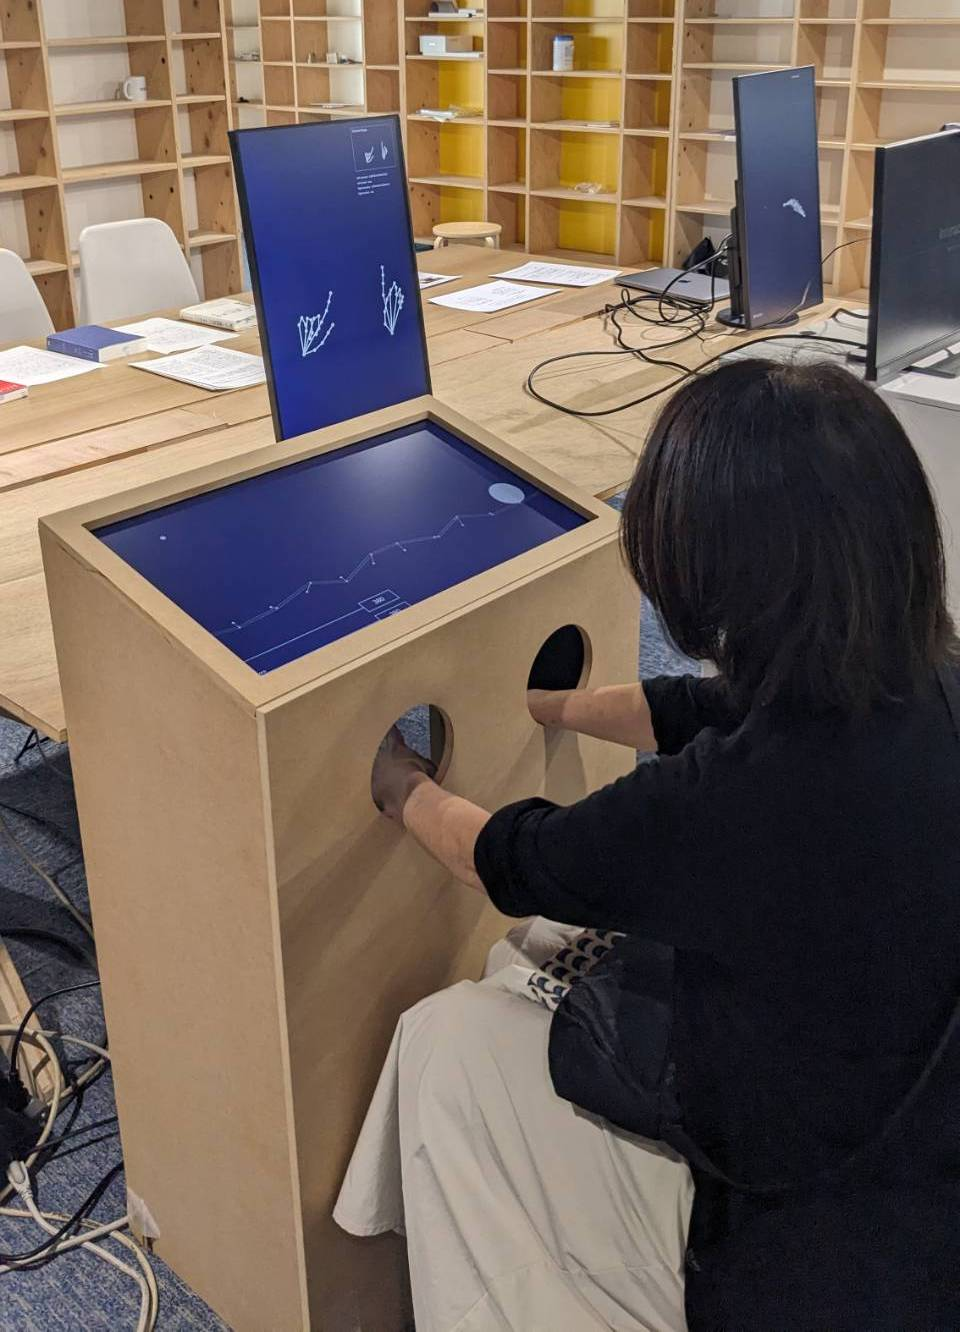
\includegraphics[width=8cm]{img/kyotai_ver1.jpg}
  \caption{中期:専用筐体を使用してカメラを隠蔽した状態}
  \label{fig:kyotai_ver1}
\end{figure}

この形式では、カメラの画角に映り込むのは筐体の内部と体験者の手のみであるため、環境光の影響や周囲の人の影響を受けずに体験できるようになった。また、穴によって手首の位置が固定されるため、腕を大きく振ることが構造上不可能となり、比較的身体動作の幅が抑えられた。

ただし、この形式は単に上記の問題を解決したというだけではなく、指先の動きが見えなくなったこと、画面に対する指先の位置関係についてを変更するものであった。

画面に対する手指の位置関係については、本作品では手指の形状が、もとの形とは全く関係のない構造へと変化するため、作品体験には大きな影響はないと判断した。手指の動きが見えなくなったことについては、画面の中の手指は体験時、自身の身体に代わる存在であるから、同時に視認できない今の形態の方がむしろ、より適した構成であると判断した。

しかしその一方で、手首の動きを固定してしまったことは、身体の動きを過剰に限定してしまう結果となった。身体の動きを限定してしまうと、何か特定の動作を求められているような説明的な構成になってしまう。そのため筐体としては、より簡素な構成が好ましいと判断した。


\textbf{作品展示:専用筐体を用いて手首を固定せず指先を自由にした状態}\\
そこで最終的には、図\ref{fig:kyotai_ver2}のような、トラッキングの範囲を暗示しながら、手首を固定しない方式に変更した。また、トラッキングに用いるカメラを、視野角150°の広角カメラ(Sanwa Supply CMS-V43BK-3)に変更し、大きく手指を動かしてもトラッキングの外れることの少ないものへと変更した。

\begin{figure}[H]
  \centering
  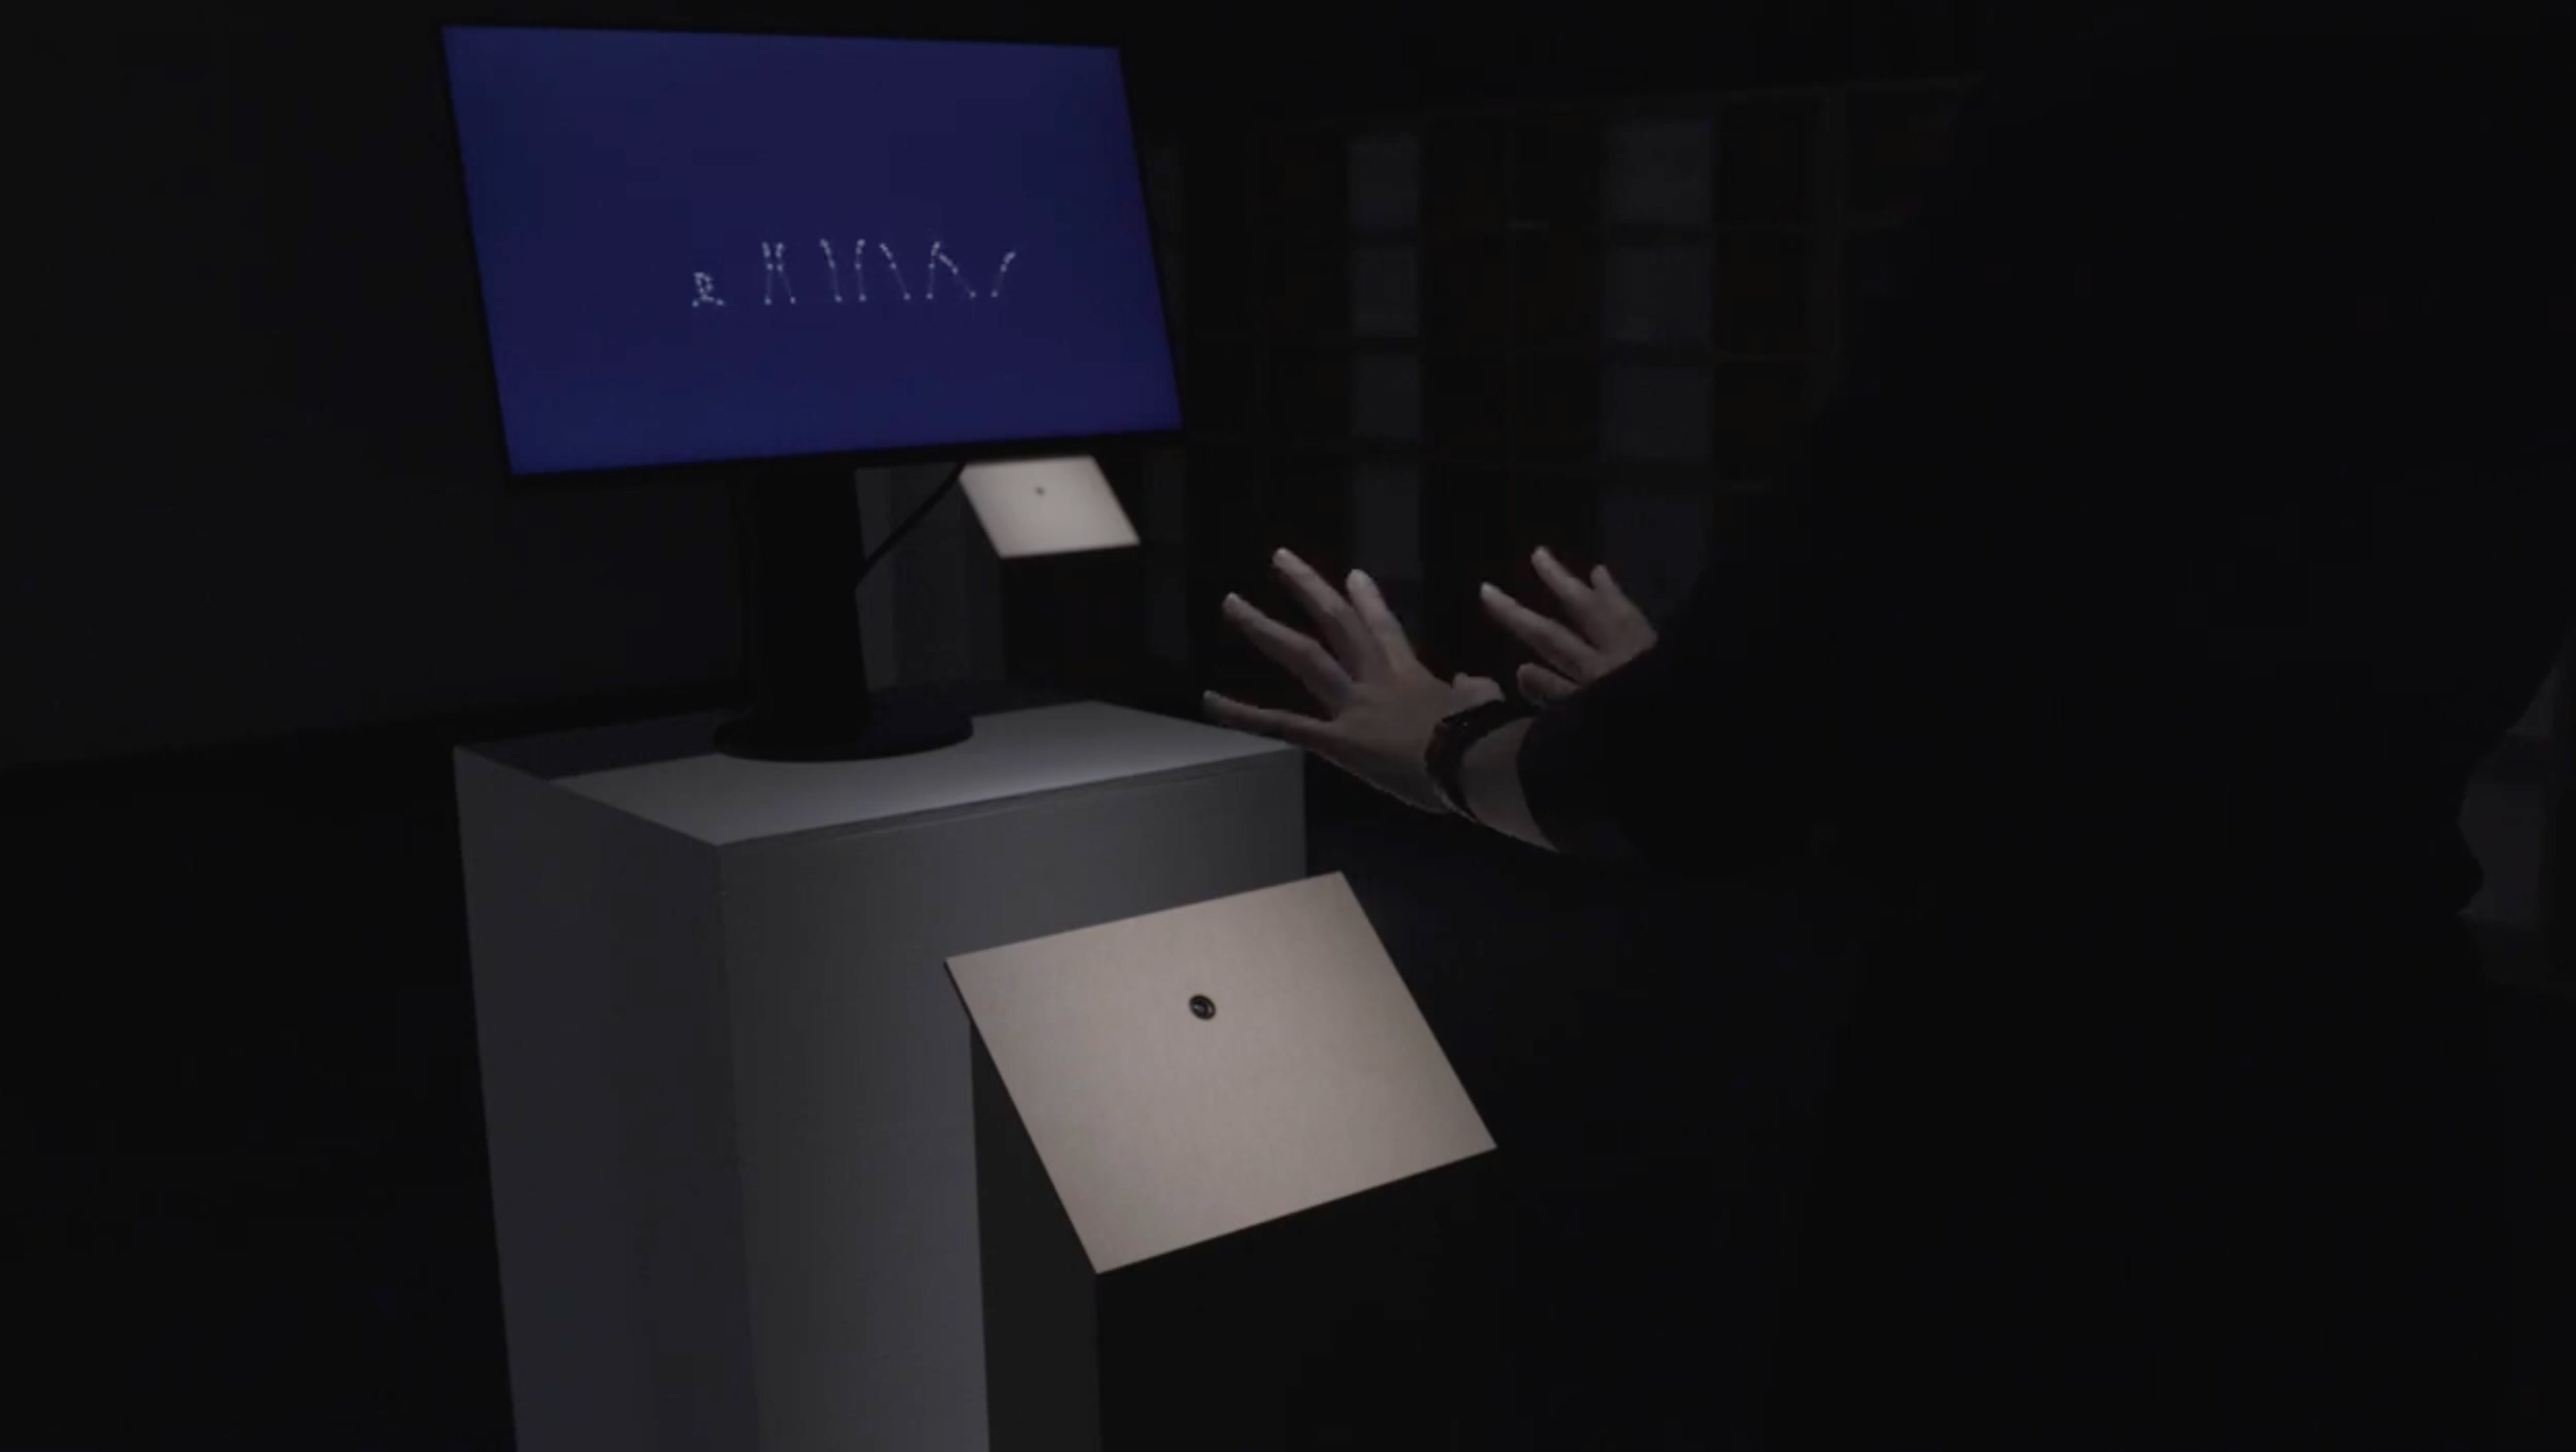
\includegraphics[width=12cm]{img/kyotai_ver2.png}
  \caption{作品展示の際の筐体}
  \label{fig:kyotai_ver2}
\end{figure}

筐体の高さは腰ほどの高さ(850mm)とすることで、キーボードのブラインドタッチのように、画面を見ながら手を同時に見ることが難しい構成とした。

カメラは、鉛直上向ではなく斜めを向いているので、筐体の前に立つと体験者の身体と手指の位置が重なり、トラッキングしやすい状況ができる。

また、ライティングの調整によってトラッキングの精度を高めた。
最終的な展示形態では、スポットライトを当てることで筐体周りを明るくすると同時に照り返しで手元の採光をし、周囲の照明を落とすことで明暗差を作ることで、手指の姿勢を認識しやすくなる。

\begin{figure}[H]
  \centering
  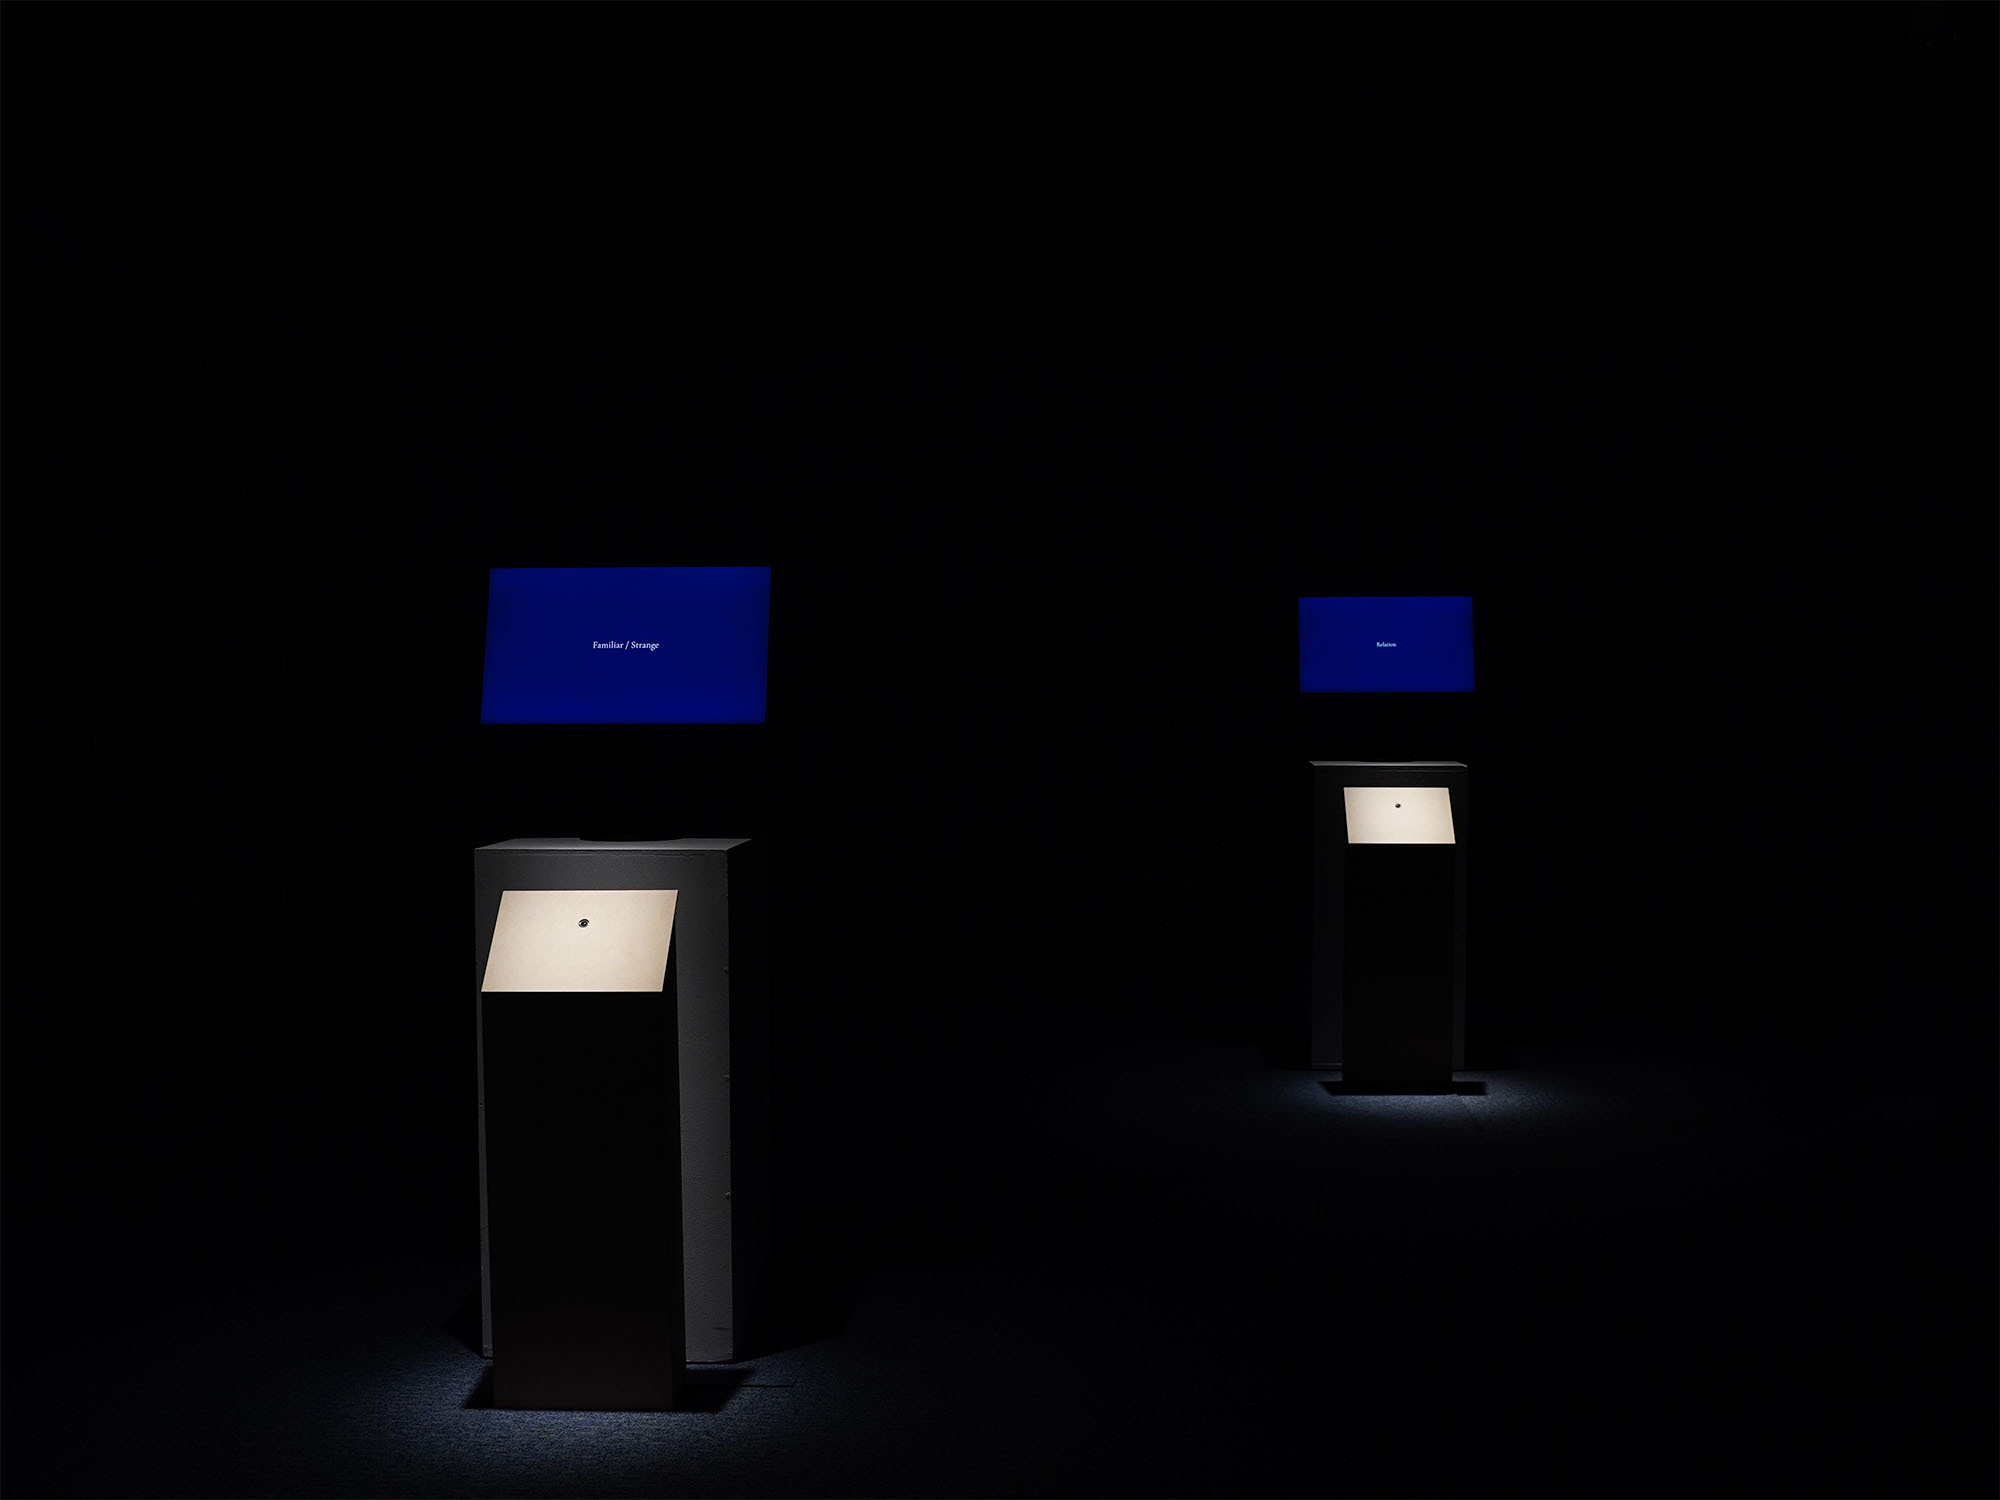
\includegraphics[width=12cm]{img/lighting.jpg}
  \caption{作品展示の際のライティング}
  \label{fig:lighting}
\end{figure}
